\documentclass[tikz,dvisvgm,border=1pt]{standalone}
% Shared preamble for the attribution infographics (iN-*.tex).
% tools/tikz-build.sh compiles each source with \variant set to wide or narrow.
\usepackage[T1]{fontenc}
\usepackage[default,semibold]{sourcesanspro}
\usepackage[italic]{mathastext}
% Larger scripts than the TeX default, so subscripts stay legible at phone width.
\DeclareMathSizes{9}{9}{8}{7}
\DeclareMathSizes{10}{10}{9}{8}
\DeclareMathSizes{11}{11}{9}{8}
\DeclareMathSizes{11.5}{11.5}{9.5}{8}
\usetikzlibrary{arrows.meta,positioning,calc,fit,backgrounds,decorations.pathreplacing,patterns}

\ifdefined\variant\else\def\variant{wide}\fi
\newif\ifnarrow
\def\narrowname{narrow}
\ifx\variant\narrowname\narrowtrue\fi
% The narrow variant is about 320pt wide and shown at about 350px, the wide one
% about 540pt wide and shown at up to 720px: the narrow one uses larger type.
\ifnarrow
  \def\basefont{\fontsize{11}{13}\selectfont}\def\smallfont{\fontsize{10}{12}\selectfont}
  \def\titlefont{\fontsize{11.5}{13.5}\selectfont\bfseries}
\else
  \def\basefont{\fontsize{10}{12}\selectfont}\def\smallfont{\fontsize{9}{11}\selectfont}
  \def\titlefont{\fontsize{11}{13}\selectfont\bfseries}
\fi

% Light-theme page tokens (web/src/styles/_variables.css, embeds.css), fixed:
% every infographic sits on its own light card, so it reads on both themes.
\definecolor{ink}{HTML}{262626}      % --text-color on white
\definecolor{muted}{HTML}{666666}    % --muted-color on white
\definecolor{rule}{HTML}{DCDCDC}     % --border-color, slightly stronger
\definecolor{surface}{HTML}{F5F5F5}  % --neutral-200
\definecolor{heading}{HTML}{904B20}  % h2 colour
\definecolor{info}{HTML}{187C9B}     % embeds --info-color
\definecolor{primary}{HTML}{C65928}  % embeds --primary-color
\definecolor{success}{HTML}{35814C}  % embeds --success-color
\definecolor{danger}{HTML}{BD3F50}   % f13 spread cost
\definecolor{residual}{HTML}{A77913} % f13 residual

\tikzset{
  every picture/.style={color=ink, line width=0.6pt, >={Stealth[length=5pt,width=4pt]},
    font=\basefont},
  small/.style={font=\smallfont},
  title/.style={font=\titlefont},
  box/.style={draw=rule, fill=white, rounded corners=4pt, align=center, inner sep=5pt},
  tag/.style={small, text=muted},
}

% No hyphenation in the narrow text columns of the diagrams.
\hyphenpenalty=10000 \exhyphenpenalty=10000

% Light card behind the whole drawing, below the background layer.
\pgfdeclarelayer{card}
\pgfsetlayers{card,background,main}
\newcommand\drawcard{%
  \begin{pgfonlayer}{card}
    \fill[white, draw=rule, rounded corners=8pt]
      ($(current bounding box.south west)+(-10pt,-10pt)$)
      rectangle ($(current bounding box.north east)+(10pt,10pt)$);
  \end{pgfonlayer}}

% Route of the page: from the order diagnostic of real-time TCA (introduction)
% to explaining a P&L, with sections 1-5 as stations and their anchors.
\begin{document}
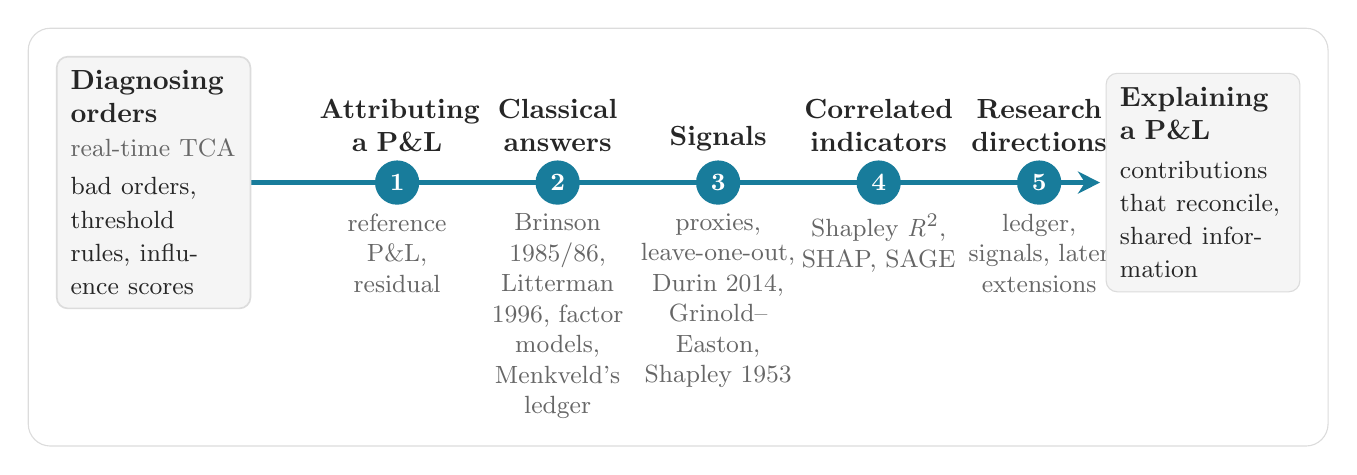
\begin{tikzpicture}
\ifnarrow
  \def\stations{%
    1/{What it means to attribute a P\&L}/{reference P\&L, residual},
    2/{The classical answers}/{Brinson 1985/86, Litterman 1996, factor models, Menkveld's ledger},
    3/{Attributing a P\&L to signals}/{proxies, leave-one-out, Durin 2014, Grinold--Easton, Shapley 1953},
    4/{Correlated indicators}/{Shapley $R^2$, SHAP, SAGE},
    5/{Research directions}/{ledger, signals, later extensions}}
  \node[box, fill=surface, text width=250pt, align=left, anchor=north west] (start) at (0,0) {%
    \textbf{Diagnosing orders} {\color{muted}(real-time TCA)}\\
    \smallfont which orders are bad, and when: threshold rules on descriptors, influence scores};
  \foreach \n/\t/\a [count=\i] in \stations {
    \coordinate (s\n) at (14pt,-26pt-\i*46pt);
    \fill[info] (s\n) circle (8pt) node[white, font=\smallfont\bfseries] {\n};
    \node[right, text width=222pt, align=left, inner sep=0pt] at ($(s\n)+(14pt,0)$)
      {\textbf{\t}\\{\smallfont\color{muted}\a}};
  }
  \begin{pgfonlayer}{background}
    \draw[info, line width=2pt] (start.south -| s1) -- (s5);
    \draw[info, line width=2pt, -{Stealth[length=8pt,width=8pt]}] (s5) -- ++(0,-24pt) coordinate (e);
  \end{pgfonlayer}
  \node[box, fill=surface, text width=250pt, align=left, anchor=north west] at (e -| start.west) {%
    \textbf{Explaining a P\&L}\\
    \smallfont contributions that reconcile, shared information};
\else
  \def\stations{%
    1/{Attributing a P\&L}/{reference P\&L, residual},
    2/{Classical answers}/{Brinson 1985/86, Litterman 1996, factor models, Menkveld's ledger},
    3/{Signals}/{proxies, leave-one-out, Durin 2014, Grinold--Easton, Shapley 1953},
    4/{Correlated indicators}/{Shapley $R^2$, SHAP, SAGE},
    5/{Research directions}/{ledger, signals, later extensions}}
  \node[box, fill=surface, text width=60pt, align=left] (start) at (0,0) {%
    \textbf{Diagnosing orders}\\{\smallfont\color{muted}real-time TCA}\\[2pt]
    \smallfont bad orders, threshold rules, influence scores};
  \foreach \n/\t/\a [count=\i] in \stations {
    \coordinate (s\n) at (30pt+\i*58pt,0);
    \fill[info] (s\n) circle (8pt) node[white, font=\smallfont\bfseries] {\n};
    \node[above=11pt of s\n, anchor=south, text width=56pt, align=center, inner sep=0pt]
      {\textbf{\t}};
    \node[below=11pt of s\n, anchor=north, text width=56pt, align=center, inner sep=0pt, small,
      text=muted] {\a};
  }
  \begin{pgfonlayer}{background}
    \draw[info, line width=2pt] (start.east) -- (s5);
    \draw[info, line width=2pt, -{Stealth[length=8pt,width=8pt]}] (s5) -- ++(22pt,0) coordinate (e);
  \end{pgfonlayer}
  \node[box, fill=surface, text width=60pt, align=left, right=2pt of e] {%
    \textbf{Explaining a P\&L}\\[2pt]
    \smallfont contributions that reconcile, shared information};
\fi
\drawcard
\end{tikzpicture}
\end{document}
